\documentclass[9pt]{beamer}

\usepackage{microtype}
\usepackage{geometry}
\usepackage[
	style=authoryear,
	citestyle=authoryear,
	maxcitenames=2,
	maxbibnames=3,
	hyperref=false,
	url=false,
	doi=false,
	isbn=false
]{biblatex}
\usepackage{amssymb}
\usepackage{booktabs}
\usepackage{graphbox}
\usepackage{graphicx}
\usepackage{tikz}

\usetikzlibrary{arrows.meta,positioning,shapes.geometric}

\usetheme{CambridgeUK}

\setbeamertemplate{navigation symbols}{}
\setbeamertemplate{headline}{}

\setbeamertemplate{enumerate items}[default]
\setbeamercolor{enumerate item}{fg=black}
\setbeamercolor{enumerate subitem}{fg=black}
\setbeamercolor{enumerate subsubitem}{fg=black}

\addbibresource{bibliography.bib}

\graphicspath{{.}{./figures/}}

\newcommand{\cop}[1]{\textsf{#1}}
\newcommand{\step}[1]{\textsf{#1}}
\newcommand{\leancop}{\cop{leanCoP}}
\newcommand{\satcop}{\cop{SATCoP}}
\newcommand{\citelogo}{
\includegraphics[width=7pt,align=c]{cite_logo.png}}
\newcommand{\sourcecite}[1]{\citelogo{} {\color{black!55}\scriptsize\parencite{#1}}}
\newcommand{\refentry}[1]{\item \fullcite{#1}}

\setbeamerfont{bibliography item}{size=\scriptsize}
\setbeamerfont{bibliography entry author}{size=\scriptsize}
\setbeamerfont{bibliography entry title}{size=\scriptsize}
\setbeamerfont{bibliography entry location}{size=\scriptsize}
\setbeamerfont{bibliography entry note}{size=\scriptsize}

\title{Reset Early, Reset Often, Eliminate Models}
\subtitle{How aggressively resetting connection tableaux can saturate the SAT solver and find an unsatisfiability proof faster.}
\author{Martin S.\ Fixman\footnotemark[1]{}, Fredrik Rømming\footnotemark[1]{}, Sean B.\ Holden\footnotemark[1]{}}
% \institute{
\includegraphics[height=10pt]{cambridge.png} \\ \footnotemark[1]{}University of Cambridge}
\institute{\raisebox{26pt}{\footnotemark[1]{}} 
\includegraphics[height=30pt]{cambridge_with_text.png} \vspace{20pt}}
\date{Vampire Workshop, FLoC 2026}

\begin{document}

\begin{frame}
	\titlepage
\end{frame}

\section{Introduction}

\begin{frame}{LeanCoP-style provers}
	\centering
	Build one connection tableau by goal-directed search.\\[5pt]
	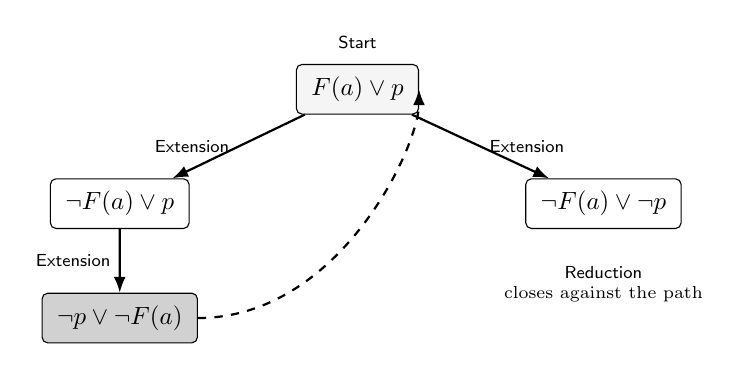
\begin{tikzpicture}[scale=.9,every node/.style={transform shape},
		clause/.style={draw,rounded corners=2pt,minimum height=7mm,inner xsep=6pt},
		label/.style={font=\scriptsize,align=center},
		flow/.style={-{Latex[length=2mm]},thick}
	]
		\node[clause,fill=black!4] (start) {$F(a) \vee p$};
		\node[label,above=1mm of start] {\step{Start}};
		\node[clause,below left=9mm and 15mm of start] (extone) {$\neg F(a) \vee p$};
		\node[clause,below=9mm of extone,fill=black!18] (exttwo) {$\neg p \vee \neg F(a)$};
		\node[clause,below right=9mm and 15mm of start] (next) {$\neg F(a) \vee \neg p$};
		\draw[flow] (start) -- node[label,left] {\step{Extension}} (extone);
		\draw[flow] (extone) -- node[label,left] {\step{Extension}} (exttwo);
		\draw[flow] (start) -- node[label,right] {\step{Extension}} (next);
		\node[label,below=4mm of next] {\step{Reduction}\\closes against the path};
		\draw[flow,dashed] (exttwo.east) .. controls +(20mm,0) and +(0,-8mm) .. (start.east);
	\end{tikzpicture}

	\vfill
	\begin{columns}[T,onlytextwidth]
		\column{.48\textwidth}
		\textbf{Proof-building rules}\\
		\step{Start}, \step{Extension}, and \step{Reduction} grow and close the tableau.

		\column{.48\textwidth}
		\textbf{Search control}\\
		Backtracking revisits choices when a locally sound connection leads to a dead end.
	\end{columns}

	\vfill
	Failed tableaux leave little information to reuse.\\[2pt]
	\sourcecite{connectiontableaux,leancop}
\end{frame}

\begin{frame}{SATCoP}
	\centering
	Keep a persistent propositional view of tableau search.\\[7pt]
	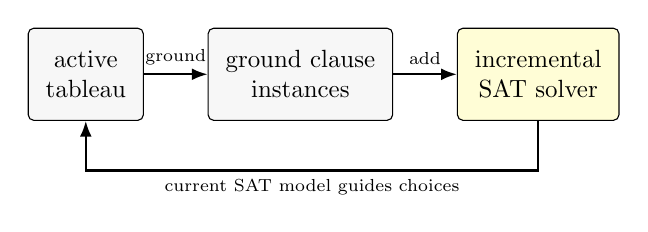
\begin{tikzpicture}[scale=.9,every node/.style={transform shape},
		node distance=9mm,
		box/.style={draw,rounded corners=2pt,minimum height=13mm,align=center,inner xsep=7pt},
		flow/.style={-{Latex[length=2mm]},thick}
	]
		\node[box,fill=black!3] (tab) {active\\tableau};
		\node[box,fill=black!3,right=of tab] (ground) {ground clause\\instances};
		\node[box,fill=yellow!16,right=of ground] (sat) {incremental\\SAT solver};
		\draw[flow] (tab) -- node[above,font=\scriptsize]{ground} (ground);
		\draw[flow] (ground) -- node[above,font=\scriptsize]{add} (sat);
		\draw[flow] (sat.south) -- ++(0,-7mm) -| node[pos=.25,below,font=\scriptsize]{current SAT model guides choices} (tab.south);
	\end{tikzpicture}

	\vfill
	\begin{columns}[T,onlytextwidth]
		\column{.47\textwidth}
		\textbf{Tableau route}\\[2pt]
		Close every open branch.

		\column{.06\textwidth}
		or

		\column{.47\textwidth}
		\textbf{SAT route}\\[2pt]
		Accumulated ground clauses become UNSAT.
	\end{columns}

	\vfill
	The SAT solver can finish the proof before the active tableau closes.\\[2pt]
	\sourcecite{satcop}
\end{frame}

\begin{frame}{Why is SATCoP so good?}
	\centering
	\cop{SYN052-1.p}: the useful result of a failed branch is no longer lost.\\[6pt]
	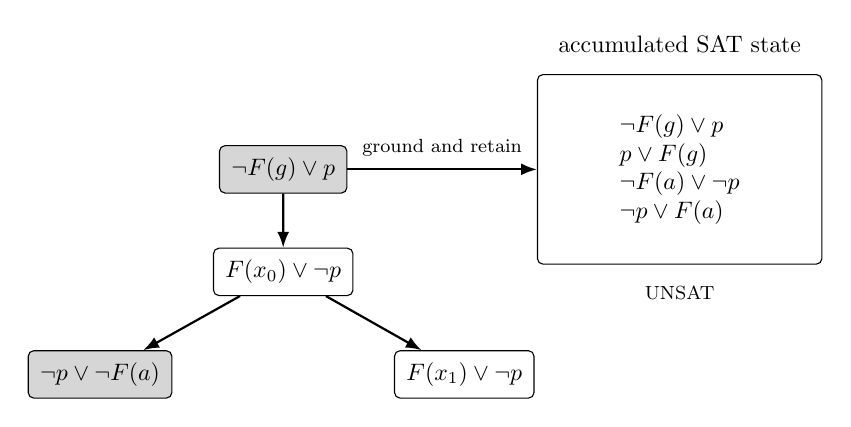
\begin{tikzpicture}[scale=.86,every node/.style={transform shape},
		clause/.style={draw,rounded corners=2pt,minimum height=7mm,inner xsep=5pt},
		core/.style={fill=black!16},
		flow/.style={-{Latex[length=2mm]},thick}
	]
		\node[clause,core] (root) {$\neg F(g) \vee p$};
		\node[clause,below=8mm of root] (child) {$F(x_0) \vee \neg p$};
		\node[clause,core,below left=8mm and 6mm of child] (left) {$\neg p \vee \neg F(a)$};
		\node[clause,below right=8mm and 6mm of child] (right) {$F(x_1) \vee \neg p$};
		\draw[flow] (root) -- (child);
		\draw[flow] (child) -- (left);
		\draw[flow] (child) -- (right);

		\node[draw,rounded corners=2pt,align=left,minimum width=42mm,minimum height=28mm,right=28mm of root] (satstate) {
			$\neg F(g) \vee p$\\
			$p \vee F(g)$\\
			$\neg F(a) \vee \neg p$\\
			$\neg p \vee F(a)$
		};
		\node[above=2mm of satstate] {accumulated SAT state};
		\draw[flow] (root.east) -- node[midway,above=1.5mm,font=\footnotesize,fill=white,inner sep=1pt]{ground and retain} (satstate.west);
		\node[below=2mm of satstate,font=\footnotesize] {UNSAT};
	\end{tikzpicture}\\[7pt]
	\begin{columns}[T,onlytextwidth]
		\column{.47\textwidth}
		\leancop: \textbf{43 steps}\\
		Must eventually close one tableau.

		\column{.47\textwidth}
		\satcop: \textbf{17 steps}\\
		Ground clauses from several attempts form an UNSAT core.
	\end{columns}

	\vfill
	\textbf{Failed search becomes useful work.}\\[2pt]
	\sourcecite{satcop}
\end{frame}

\begin{frame}{Improvements to SATCoP}
	\centering
	\satcop{} makes the SAT solver part of search control.\\[8pt]
	\small
	\begin{tabular}{lccc}
		\toprule
		& SAT refutation & SAT-model guidance & Local backtracking \\
		\midrule
		\leancop{} & & & \checkmark \\
		\satcop{}  & \checkmark & \checkmark & \checkmark \\
		\bottomrule
	\end{tabular}

	\vfill
	\begin{columns}[T,onlytextwidth]
		\column{.48\textwidth}
		\begin{block}{Explore more broadly}
			Randomise starts, extension choices, and clause-literal order.
		\end{block}

		\column{.48\textwidth}
		\begin{block}{Follow the SAT model}
			Prefer extensions whose selected literal is true in the current model.
		\end{block}
	\end{columns}

	\vfill
	The SAT solver needs diverse ground clauses; local backtracking keeps exploring near the same tableau choices.\\[2pt]
	\sourcecite{satcop,leancopcut,connections_2023}
\end{frame}

\section{SATResetCoP}
\begin{frame}{What if we stop doing regular tableau guidance?}
	\centering
	When an attempt stops producing new ground clauses, use \step{Reset} instead of \step{Backtrack}.\\[7pt]
	\begin{tikzpicture}[scale=.9,every node/.style={transform shape},
		clause/.style={draw,rounded corners=2pt,minimum height=7mm,inner xsep=5pt},
		core/.style={fill=black!16},
		flow/.style={-{Latex[length=2mm]},thick}
	]
		\node[clause,core] (leftroot) {$\neg F(g) \vee p$};
		\node[clause,below=8mm of leftroot] (leftchild) {$F(x_0) \vee \neg p$};
		\node[clause,below=8mm of leftchild] (leftleaf) {$F(x_1) \vee \neg p$};
		\draw[flow] (leftroot) -- (leftchild);
		\draw[flow] (leftchild) -- (leftleaf);

		\node[clause,core,right=50mm of leftroot] (rightroot) {$p \vee F(g)$};
		\node[clause,core,below=8mm of rightroot] (rightchild) {$\neg p \vee \neg F(a)$};
		\node[clause,core,below=8mm of rightchild] (rightleaf) {$F(a) \vee \neg p$};
		\draw[flow] (rightroot) -- (rightchild);
		\draw[flow] (rightchild) -- (rightleaf);

		\draw[flow,cambridgeorange] (leftroot.east) -- node[midway,above=2mm,text=black,fill=white,inner sep=1pt]{\step{Reset}} (rightroot.west);
		\node[below=4mm of rightleaf,font=\footnotesize] {UNSAT core reached};
	\end{tikzpicture}\\[7pt]
	\begin{columns}[T,onlytextwidth]
		\column{.47\textwidth}
		\satcop: \textbf{17 steps}\\
		Run \step{Backtrack} through the current tableau.

		\column{.47\textwidth}
		\cop{SATResetCoP}: \textbf{6 steps}\\
		Run \step{Reset} to expose the UNSAT core faster.
	\end{columns}

	\vfill
	Use tableaux as \textbf{ground-clause generators} for SAT.\\[2pt]
	\sourcecite{satcop}
\end{frame}

\begin{frame}{SATResetCoP}
	\centering
	Guide tableau search to saturate the incremental SAT solver.\\[2pt]
	\sourcecite{connections_2023,cadical20}\\[6pt]
	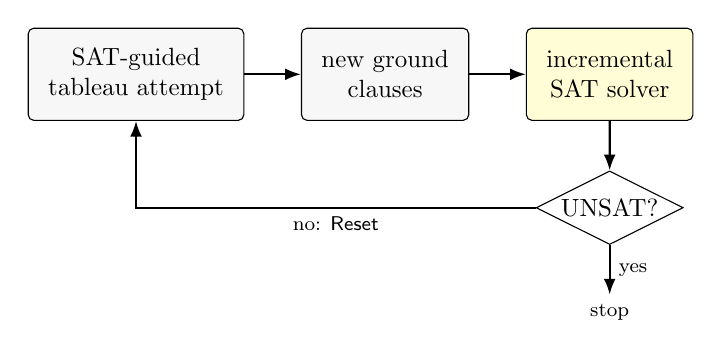
\begin{tikzpicture}[scale=.9,every node/.style={transform shape},
		node distance=8mm,
		box/.style={draw,rounded corners=2pt,minimum height=13mm,align=center,inner xsep=8pt},
		decision/.style={draw,diamond,aspect=2,align=center,inner sep=1pt},
		flow/.style={-{Latex[length=2mm]},thick}
	]
		\node[box,fill=black!3] (attempt) {SAT-guided\\tableau attempt};
		\node[box,fill=black!3,right=of attempt] (clauses) {new ground\\clauses};
		\node[box,fill=yellow!16,right=of clauses] (solver) {incremental\\SAT solver};
		\draw[flow] (attempt) -- (clauses);
		\draw[flow] (clauses) -- (solver);
		\node[decision,below=7mm of solver] (unsat) {UNSAT?};
		\draw[flow] (solver) -- (unsat);
		\draw[flow] (unsat.south) -- node[right,font=\footnotesize]{yes} ++(0,-7mm)
			node[below,font=\footnotesize]{stop};
		\draw[flow] (unsat.west) -| node[pos=.25,below,font=\footnotesize]{no: \step{Reset}} (attempt.south);
	\end{tikzpicture}

	\vfill
	\begin{columns}[T,onlytextwidth]
		\column{.31\textwidth}
		\textbf{Choose}\\
		Randomise starts and extensions; prefer literals supported by the SAT model.

		\column{.31\textwidth}
		\textbf{Accumulate}\\
		After \step{Extension} and \step{Reduction}, collect genuinely new ground clauses.

		\column{.31\textwidth}
		\textbf{\step{Reset}}\\
		At a dead end, flush new clauses and run \step{Reset}; increase depth only after no progress.
	\end{columns}
\end{frame}

\section{Results}
\begin{frame}{General Results}
	\centering
	\begin{columns}[c,onlytextwidth]
		\column{.61\textwidth}
		\textbf{TPTP problems solved}\\[5pt]
		\begin{tikzpicture}[x=.0105mm,y=9mm]
			\node[anchor=e] at (-80,2.3) {\leancop};
			\fill[cambridgelightblue] (0,2) rectangle (1923,2.6);
			\node[anchor=west] at (1983,2.3) {1,923};

			\node[anchor=e] at (-80,1.3) {\satcop};
			\fill[cambridgeblue] (0,1) rectangle (2509,1.6);
			\node[anchor=west] at (2569,1.3) {2,509};

			\node[anchor=e] at (-80,.3) {\cop{SATResetCoP}};
			\fill[cambridgeorange] (0,0) rectangle (2971,.6);
			\node[anchor=west] at (3031,.3) {2,971};
		\end{tikzpicture}

		\column{.35\textwidth}
		\textbf{MPTP2078}\\[3pt]
		{\Large 616 problems}\\[4pt]
		\textbf{+12\%} over \satcop{}\\
		\textbf{+49\%} over \leancop{}
	\end{columns}

	\vfill
	\textbf{Aggressive \step{Reset}s solve more problems, usually in fewer steps.}\\[2pt]
	\scriptsize 120 seconds and 1 million tableau steps per problem. The \step{Reset} policy also loses 136 TPTP problems solved by \satcop{}: a schedule should keep both search modes.\\[2pt]
	\sourcecite{tptp,mptp2078}
\end{frame}

\section{References}
\begin{frame}{References}
	\scriptsize
	\begin{columns}[T,onlytextwidth]
		\column{.48\textwidth}
		\begin{itemize}\setlength{\itemsep}{5pt}
			\refentry{connectiontableaux}
			\refentry{leancop}
			\refentry{leancopcut}
			\refentry{satcop}
		\end{itemize}

		\column{.48\textwidth}
		\begin{itemize}\setlength{\itemsep}{5pt}
			\refentry{connections_2023}
			\refentry{cadical20}
			\refentry{tptp}
			\refentry{mptp2078}
		\end{itemize}
	\end{columns}
\end{frame}
	
\end{document}
